\documentclass[a4paper,12pt]{article}
\usepackage[left=2.5cm, top=2cm, right=1.5cm, bottom=2cm]{geometry}

%%% Работа с русским языком
\usepackage{cmap}					% поиск в PDF
\usepackage{mathtext} 				% русские буквы в формулах
\usepackage[T2A]{fontenc}			% кодировка
\usepackage[utf8]{inputenc}			% кодировка исходного текста
\usepackage[english,russian]{babel}	% ло кализация и переносы
%%\usepackage{textcomp}

%%% Дополнительная работа с математикой
\usepackage{amsmath,amsfonts,amssymb,amsthm,mathtools} 
%\usepackage{textcomp}

%% Номера формул
\usepackage{xymtexpdf}
\usepackage{chmst-pdf}

%%% Работа с картинками
\usepackage{graphicx}  % Для вставки рисунков
\usepackage{rotating}
\setlength\fboxsep{3pt} % Отступ рамки \fbox{} от рисунка
\setlength\fboxrule{1pt} % Толщина линий рамки \fbox{}
\usepackage{wrapfig} % Обтекание рисунков текстом

%%% Работа с таблицами
\usepackage{array,tabularx,tabulary,booktabs} % Дополнительная работа с таблицами
\usepackage{longtable}  % Длинные таблицы
\usepackage{multirow} % Слияние строк в таблице


%%% Программирование

%%%tikz
\usepackage{tikz}
\usetikzlibrary{calc}
\usetikzlibrary{patterns}
\usetikzlibrary{shadows}
\usepackage{indentfirst} % Красная строка


\usepackage[os=win, mackeys=symbols]{menukeys}
\usepackage{enumitem}
\usepackage{hyperref}
\usepackage[russian,noabbrev]{cleveref}

\graphicspath{{fig/}}

\usepackage{lastpage}
\usepackage{fancyhdr}


\usepackage{xassoccnt}
\NewTotalDocumentCounter{totalfigures}
\NewTotalDocumentCounter{totaltables}
\NewTotalDocumentCounter{appendixchapters}
\DeclareAssociatedCounters{figure}{totalfigures}
\DeclareAssociatedCounters{table}{totaltables}
\NewTotalDocumentCounter{totalpages}
\NewDocumentCounter{realpages}
\DeclareAssociatedCounters{page}{totalpages}

\makeatletter
\AtBeginDocument{%
	\stepcounter{realpages}%
}
\EveryShipout{%
	\stepcounter{realpages}%
}
\AtEndDocument{%
	\setcounter{xassoccnt@total@totalpages}{\value{realpages}}%
	\write\@auxout{%
		\string\setcounter{xassoccnt@total@totalpages}{\number\value{realpages}}%
	}
}
\makeatother


\usepackage{listings}
\usepackage{color}

\usepackage[toc,page]{appendix}

%%% Заголовок
\author{Ivan Anashkin}
\title{rfbr}
\date{\today}

\begin{document}
\begin{center}
	\textsc{\large{Министерство науки и высшего образования Российской Федерации}\\
	\footnotesize{Федеральное государственное бюджетное образовательное учреждение высшего образования}\\ 
	\small{\textbf{«Казанский национальный исследовательский технологический университет»}}\\}
\end{center}

	\hfill \break
	\normalsize{УДК: 544.272:66.011}\\
	\normalsize{№ Госрегистрации \textbf{АААА-А18-118032690262-8}}\\
	\normalsize{Инв. №}\\
	
	\large
	~\hspace{9cm}\textsc{Утверждаю}
	
	~\hspace{7cm} Проректор по научной работе
	
	~\hspace{7cm}\underline{\hspace{3cm}} Сабирзянов А.Н.
	
	~\hspace{7cm}<<\underline{\hspace{1cm}}>> \underline{\hspace{4cm}} г.
	
	\hfill \break
\begin{center}
	\Large{Отчет о научно~-- исследовательской работе}\\
	\hfill \break
	\Large{по теме: Молекулярно~-- статистическое моделирование процесса ректификации\\(промежуточный)}\\
	\hfill \break
	\hfill \break
	\normalsize
	\large
Руководитель темы:\hspace{5cm}   \underline{\hspace{2.7cm}} Анашкин И.П.
\hfill \break
\vspace{8cm}
\hfill \break
 Казань 2019
\end{center}
\thispagestyle{empty} % выключаем отображение номера для этой страницы


\newpage

\section*{Список исполнителей:}
\normalsize{ 
	\begin{tabular}{cccc}
		Руководитель проекта & \hspace{3cm} &  \underline{\hspace{3cm}} & Анашкин И.П. \\\\
		\hfill \break
		Исполнители: &  & \underline{\hspace{3cm}} & Казанцев С.В. \\\\
	\end{tabular}
\thispagestyle{empty} % выключаем отображение номера для этой страницы

\newpage
\section*{Реферат}
страниц -- \TotalValue{totalpages}

рисунков -- \TotalValue{totalfigures}

таблиц -- \TotalValue{totaltables}

приложений -- 1 %\TotalValue{appendixchapters}

Ключевые слова: ректификация, метод Монте-Карло, межмолекулярное взаимодействие
\thispagestyle{empty}
\newpage

\tableofcontents

\thispagestyle{empty}

\newpage


	
\addcontentsline{toc}{section}{Введение}
\subsection*{Введение}

Ректификация --- один из наиболее распространенных процессов разделения смесей, применяемых в химической промышленности. Для расчета процесса ректификации разработано множество подходов, в основе которых лежит использование данных о фазовом равновесии компонентов разделяемой смеси. Поэтому, расчетную схему ректификационной колонны необходимо дополнить моделями для описания давления насыщенных паров чистых компонентов и коэффициентов активности в смеси. Однако экспериментальные данные доступны не для всех комбинаций веществ, или доступны в ограниченной области состояний. Решением может выступать использование методов групповых составляющих \cite{Skjold-Jorgensen1979,Tiegs1987,Wittig2003}, однако данные методы не гарантируют хорошего согласования с экспериментальными данными.

В данной работе предлагается использование молекулярно-статистических методов для моделирования процесса ректификации. В основе предлагаемого подхода лежит использование законов сохранения, метода теоретических тарелок и метода ансамбля Гиббса для вычисления фазового равновесия.

\section{Молекулярно-статистический метод расчета процесса ректификации}



\subsection{Молекулярно-статистические методы и программные пакеты}

В настоящее время молекулярно~-- статистические методы находят широкое применение в научных исследованиях в различных отраслях. Данные методы позволяют на молекулярном уровне исследовать свойства веществ, а также процессов, происходящих на молекулярном уровне. Для проведения моделирования разработано множество пакетов программ, отличающихся функциональностью и условиями предоставления программ \cite{wiki_progs}. Множество программных продуктов создано под коммерческой лицензией, например, Material Studio \cite{material_studio} , Materials Science Suite \cite{shedinger} и т.~д. Данные программные продукты нацелены на широкое применение во многих областях, что зачастую плохо сказывается на производительности их вычислений. Однако в них есть свой интерфейс пользователя, что существенно снижает порог вхождения и простоту для конченного потребителя.

Если сравнивать два подхода молекулярного моделирования: метод молекулярной динамики и метод Монте~-- Карло, и их модификации --- то наибольшее распространение получил метод молекулярной динамики. В первую очередь это связано с тем, что данный метод позволяет получить кинетические характеристики, такие как коэффициенты диффузии, вязкости и т.~д. Также сравнивая алгоритмы расчета, метод молекулярной динамики позволяет более эффективно использовать параллельные расчеты на нескольких вычислительных ядрах. Данный факт также способствовал большему распространению вычислений с использованием метода молекулярной динамики. Среди программ с открытым исходным кодом можно выделить gromacs \cite{Berendsen1995,Pronk2013,Abraham2015} и LAMMPS \cite{Plimpton1995,Thompson2009} . Данные программы получили широкое распространение за счет открытого исходного кода и большого количества заинтересованных разработчиков, что привело к отличной вычислительной производительности, в том числе на специфическом оборудовании. 

Метод Монте-Карло при моделировании классических (не квантовых систем) также обладает своими преимуществами. Например, проще реализовано вычисление химического потенциала системы, что позволяет проще производить вычисления фазового равновесия. Так, для вычисления фазового равновесия разработан ансамбль Гиббса \cite{Panagiotopoulos1987,Orkoulas1994}. Среди программного обеспечения с открытым исходным кодом можно выделить towhee \cite{Martin2013}. Данная программа изначально разрабатывалась для моделирования паро~-- жидкостного равновесия и содержит множество наборов параметров для моделирования. Недостатком данного пакета является то, что во времена начала разработки данной программы не были распространены многопроцессорные компьютеры и многоядерные процессоры. Таким образом данный пакет не позволяет в полной мере использовать все достоинства многопоточного вычисления.



\subsection{Многопоточное вычисление и программно-аппаратная технология CUDA}
Использование молекулярно-статистических методов непосредственно связано с развитием вычислительных технологий еще с разработки первых ЭВМ \cite{Allen1988}. Рассматривая развитие персональных компьютеров можно сказать, что увеличение вычислительных мощностей до середины 2000-х годов продолжалось в большей степени за счет наращивания частоты процессора. Однако накладываемые технологические ограничения не позволили превысить номинальную частоту в 4 ГГц для центрального процессора. В 2005 году на рынок выпускают процессор, содержащий два ядра. В дальнейшем происходит тенденция к наращиванию количества ядер в процессоре. Параллельно с этим развиваются программные средства, позволяющие использовать множество потоков для вычисления.

В 2008 году была представлена программно~-- аппаратная технология CUDA использующая для вычислений процессор видеокарты. Отличие от центрального процессора заключается в том, что видеокарта имеет множество специализированных процессоров, их количество в современных видеокартах достигает нескольких тысяч. Данная технология позволяет увеличить производительность для отдельных задач в несколько десятков и сотен раз. Позже появилась аналогичная технология OpenCL, не привязанная к оборудованию конкретного производителя.

В задачах молекулярной динамики использование видеокарт для расчета приводит к увеличению производительности в 10 раз по сравнению с использованием только центрального процессора. Данные технологии реализованы во многих программных продуктах \cite{wiki_progs}.

\subsection{Ансамбль Гиббса} \label{p.gibbs}
Для того чтобы две фазы (обозначенные I и II) находились в равновесии необходимо выполнение следующих условий:
\begin{itemize}
	\item термическое равновесие (равенство температур) $T^I = T^{II}$;
	\item механическое равновесие (равенство давлений) $p^I = p^{II}$;
	\item химическое равновесие (равенство химического потенциала каждого из компонентов) $\mu_i^I = \mu_i^{II}$.
\end{itemize}

Метод ансамбля Гиббса предусматривает моделирование двух ячеек с молекулами. В каждой из ячеек происходит три типа случайных изменений конфигурации:
\begin{itemize}
	\item перемещение молекулы внутри каждой ячейки (перемещение, вращение, изменение внутренней геометрии молекулы);
	\item изменение объемов каждой из ячейки;
	\item перемещение молекул между ячейками.
\end{itemize}
После каждого изменения конфигурации рассчитывается вероятность принятия или отклонения данного изменения. После значительного количества перемещений между двумя ячейками устанавливается равновесие. 


\subsection{Алгоритм расчета ректификации}
Согласно предлагаемому методу, ректификационная колонна делится на участки, аналогичные теоретическим тарелкам (теоретическим ступеням). Каждая из тарелок делится на две ячейки, которые соответствуют газовой и жидкой фазам. Суммарный объем газовой и жидкой фазы на каждой из тарелок остается постоянным. С точки зрения конструкции колонны данный указанный суммарный объем характеризует объем колонны между тарелками.При проектировании могут применяться колонны с переменным диаметром, что обеспечивает равномерность газовой фазы по высоте колонны. Таким образом, в алгоритме суммарный объем каждой из ячеек может быть задан любой, однако он не меняется во время моделирования.

На тарелке между газовой и жидкой фазами устанавливается фазовое равновесие, рассчитываемое методом ансамбля Гиббса (раздел \ref{p.gibbs}). После достижения фазового равновесия жидкость уходит на нижнюю тарелку, пар поднимается на верхнюю. Молекулы переносят свою энергию (кинетическую и потенциальную) и исходя из этой энергии проводится пересчет температуры на новой тарелке. И расчетный цикл повторяется --- заново рассчитывается фазовое равновесие. 

Таким образом в колонне можно проследить за материальными (количество молекул каждого из веществ) и тепловыми потоками (энергия молекул). Также в колонне можно выделить внешние материальные и тепловые потоки: приток молекул с исходной смесью, и флегмой, уход молекул с дистиллятом и кубовым остатком.

Блок-схема алгоритма расчета представлена на рисунке \ref{fig:alg_scheme}. На первом этапе проводится чтение исходных данных для моделирования. Далее рассчитываются свойства входящих материальных потоков. При условии, что колонна работает в стационарном режиме, свойства входящих потоков не должны изменяться. И данную процедуру необходимо провести только один раз на начальном этапе. Однако можно предусмотреть динамическое изменение исходного состава. В этом случае вычисление входящих материальных потоков необходимо включить в расчетный цикл.

\begin{figure}
	\begin{center}
		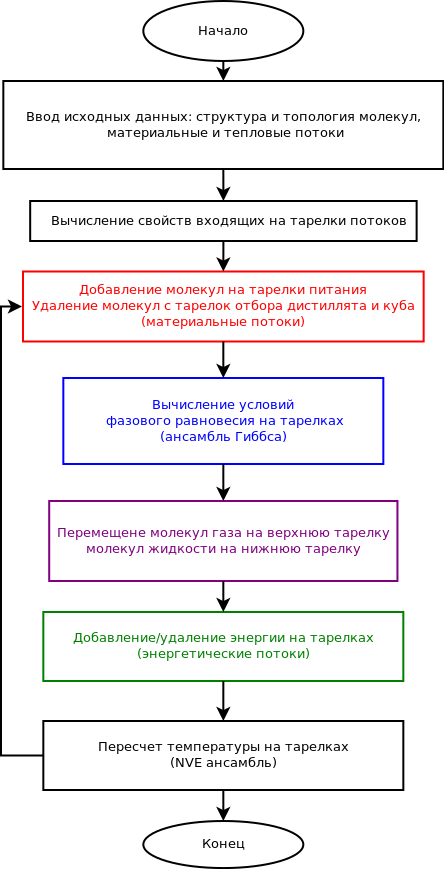
\includegraphics[width=0.5\textwidth]{scheme.png}
	\end{center}
	\caption{Блок-схема алгоритма расчета} \label{fig:alg_scheme}
\end{figure}

Далее рассчитываются внешние материальные потоки (красный блок): добавляется заданное количество молекул на тарелку питания, рассчитывается количество молекул во флегме, а также количество молекул, выводимых из куба.

Далее вычисляются условия фазового равновесия на каждой тарелке с использованием ансамбля Гиббса (синий блок).

После установления фазового равновесия на всех тарелках происходит обмен молекулам между тарелками. Жидкая фаза переходит на нижнюю тарелку, газовая фаза переходит на верхнюю тарелку (фиолетовый блок).

На каждую из тарелок можно вводить дополнительные энергетические потоки: подогрев куба колонны, введение дополнительных змеевиков охлаждения и т.д. (зеленый блок)

После перемещения молекул на каждой из тарелок вычисляется температура по внутренней энергии газовой и жидкой фаз (черный блок). Суммарная энергия молекул на тарелке высчитывается как кинетическая и потенциальная энергия молекул газовой и жидкой фаз. Кинетическая энергия может быть вычислена из температуры на тарелке, потенциальная --- как сумма межмолекулярного и внутримолекулярного (потенциал валентных и торсионных углов и т.д.) взаимодействия.
Новая температура на тарелке может быть вычислена из энергии молекул на тарелке с использованием ансамбля с постоянным количеством молекул, объемом и энергией $NVE$ \cite{Lustig1998}.

Альтернативный алгоритм определения температуры основан на одновременном изменении температуры во время вычисления фазового равновесия. В данном случае блок добавления энергии будет выполнен раньше, чем расчет условий фазового равновесия. Во время вычисления фазового равновесия температура на тарелке будет динамически изменяться таким образом, чтобы энергия системы была равна сумме энергий поступающих на тарелку молекул с газовой и жидкой фазой и энергетических потоков. Выбор конкретной из описанных выше  реализаций алгоритма определения температуры будет осуществляться на этапе программирования.
 
Далее алгоритм циклически повторяется до достижения условия стационарности, или любого другого заданного условия. Например при периодической ректификации может быть задано количество оставшейся жидкости в кубе, при этом будет исследован неравновесный процесс.
 
На рисунке \ref{fig:plate_scheme} представлено схематическое распределение потоков в ректификационной колонне. Цвет стрелок и текста соответствует различным этапам алгоритма, представленного на рисунке \ref{fig:alg_scheme}


\begin{figure}[h]
	\begin{center}
		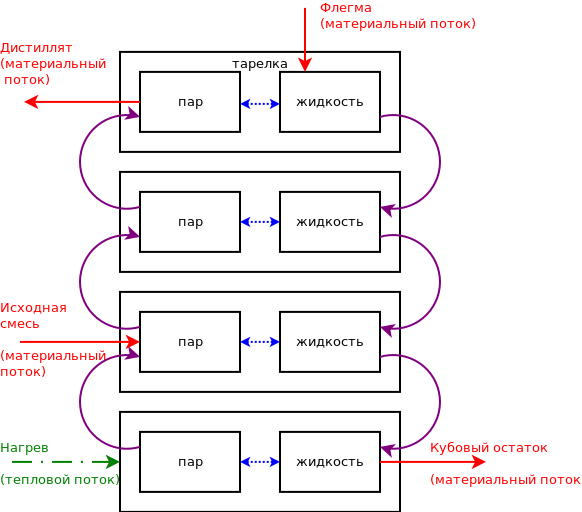
\includegraphics[width=0.7\textwidth]{column.png}
	\end{center}
	\caption{Схематическое изображение ректификационной колонны (цвет соответствует различным этапам, представленным на рисунке \ref{fig:alg_scheme})} \label{fig:plate_scheme}
\end{figure}

Усреднение свойств смеси на тарелках и выходных потоках (концентрации, температуры, давления и т.д.) проводится после установления стационарности. Достижение стационарности можно отследить по неизменности составов и количества молекул на каждой тарелке.

Достоинства предлагаемого алгоритма расчета:
\begin{itemize}
	\item не нужно заранее знать фазовое равновесие разделяемых компонентов;
	\item расчет ведется с учетом непостоянства мольных потоков по колонне;
	\item возможность исследования как непрерывной так и периодической ректификации;
	\item преимущества при расчете многокомпонентной ректификации (при недостатке экспериментальных данных), т.к. фазовое равновесие рассчитывается на каждой тарелке при своих условиях. 
\end{itemize}
Недостатками является то, что данный метод не учитывает эффективность тарельчатых устройств реальных аппаратов, обусловленной гидродинамической обстановкой. Данную проблему можно решить в будущем.



\section{Программная реализация}
Исходный код программы доступен в репозитории открытых проектов github  по ссылке \cite{github_mcr}. Текущая ветка разработки doublebox. В качестве системы сборки приложения используется Cmake. Для увеличения производительности программы разработка велась на языке CUDA. Библиотеки для осуществления многопоточных рачетов на центральном процессоре не осуществлялись в связи с тем, что на центральном процессоре осуществляется лишь небольшая часть вычислений, связанная с подготовкой исходных данных.

\subsection{Ввод исходных данных}
Для проведения моделирования необходимо задать исходные данные, что является первым этапом на схеме \ref{fig:alg_scheme}. Исходныост невозможно - по всему Интернету теперь в каждой статье перечислены ровно все те же самые баззворды, но на полностью серьёзных щах.е данные были разделены на три типа: 
\begin{itemize}
	\item исходные параметры моделирования (количество материальных потоков, составы и т.д.) хранятся в файле <<data.mcr>>;
	\item положение атомов в каждом из типов молекул хранятся в фалах <<name.gro>> (название файла должно соответствовать данным введенным в файл <<data.mcr>>);
	\item  топология молекул (параметры внутри и межмолекулярного взаимодействия) хранятся в файле <<data.top>>.
\end{itemize}


Файл <<data.mcr>> содержит параметры моделирования. Пустые строки и строчки начинающиеся с символа <<\#>> игнорируются как комментарии. В каждой строке указан один из параметров моделирования:
\begin{itemize}
	\item substance\_number -- количество веществ в исходной смеси
	\item substance\_files -- в строке указывается последовательно название <<.gro>> файлов с координатами молекул 
	\item input\_flows -- количество входящих материальных потоков в колонну
	\item input\_ensamble -- ансамбль моделирования для каждого исходного потока (пока поддерживается nvt ансамбль)
	\item input\_temperature -- температура в Кельвинах для каждого потока
	\item input\_density -- плотность потока в моль.л для каждого потока
	\item input\_ins\_mol -- количество молекул каждого из компонентов добавляемых в поток
	\item plates\_number -- количество тарелок в моделируемой колонне
	\item plates\_init -- тип начального заполнения колонны. На текущий момент в качестве параметра можно использовать только vak. Данная опция означает что изначально колонна является пустой. А дальнейшем планируется реализация заполнения газом (интертным газом или воздухом заданного давления).
	\item plates\_ins\_number -- номер тарелки поступает исходный поток
	\item plates\_vol -- объем тарелки (двух ячеек газовой и жидкой фаз) в нм$^3$
	
\end{itemize}

Пример файла с параметрами моделирования:
\begin{lstlisting}
	#substance properties
	substance_number = 2
	substance_files  =  A.gro	B.gro
	
	#material flow properties
	input_flows = 1
	input_ensamble = nvt
	input_temperature = 1.0
	input_density = 30.7616586686354
	input_ins_mol = 200 200
	
	#plates properties
	plates_number = 6
	plates_init = vak
	plates_ins_number = 3
	plates_insertion = true
	plates_vol = 2000.0    #nm-3

	#initial state
\end{lstlisting}

В разрабатываемой программе реализована совместимость с форматом файлов пакета gromacs (файлы разрешения <<gro>> и  <<top>>). Файлы с координатами атомов имеют вид:
\begin{lstlisting}
MD of 2 waters, t= 0.0
3
1WATER  OW1    1   0.126   1.624   1.679  0.1227 -0.0580  0.0434
1WATER  HW2    2   0.190   1.661   1.747  0.8085  0.3191 -0.7791
1WATER  HW3    3   0.177   1.568   1.613 -0.9045 -2.6469  1.3180
1.82060   1.82060   1.82060
\end{lstlisting}

Первая строка является комментарием, во второй указано количество атомов в молекуле (или во всей системе). Далее идет информация по каждому атому: номер молекулы, название молекулы, номер атома, $x$, $y$, $z$ координаты, $\upsilon_x$,  $\upsilon_y$, $\upsilon_z$ компоненты скорости. В последней строчке указаны размеры ячейки (эта строчка в данной программе не используется).

Файл топологии имеет вид:
\begin{lstlisting}
[ defaults ]
1    2 no    1.00000   1.00000
[ atomtypes ]
Si    28.0000    0.9000 A    0.38264   1.25700
C2   14.0000   -0.2250 A    0.39500   0.38244
O    16.0000   -0.4500 A    0.31181   0.62850
CE1    15.0110    0.0000 A    0.36072   0.99898
CE2    14.0110    0.2526 A    0.34612   0.71746
OE1    15.9994   -0.6971 A    0.31496   0.70717
HE1     1.0080    0.4415 A    0.01000   0.00000
[ bondtypes ]
CE1    CE2      1        0.19842   500000.00000
CE2    OE1      1        0.17158   500000.00000
OE1    HE1      1        0.09505   500000.00000
OW     HW      1        0.09572   500000.00000
OW     MW      1        0.01546   500000.00000
[ angletypes ]
CE1    CE2    OE1      1  90.95000 500.00000
CE2    OE1    HE1      1 106.36800 500.00000
HW     OW     HW       1 104.52000 500.00000
MW    OW    HW       1  52.26000 500.00000
[ dihedraltypes ]
CE1    CE2    OE1    HE1      5   5.00000   0.00000   0.00000   0.00000

[ moleculetype ]
ETH  3
[ atoms ]
1  CE1      1 ETH CE1    1   0.00000  15.01100
2  CE2      1 ETH CE2    1   0.25560  14.01100
3  OE1      1 ETH OE1    1  -0.69711  15.99940
4  HE1      1 ETH HE1    1   0.44151   1.00800
[ bonds ]
1    2    1
2    3    1
3    4    1
[ pairs ]
[ angles ]
1    2    3    1
2    3    4    1
[ dihedrals ]
1    2    3    4    5
[ exclusions ]
[ position_restraints ]
[ constraints ]

[ system ]
generateg
[ molecules ]
ETH    1000
\end{lstlisting}

В квадратных скобках указаны ключевые слова, после которых идет определенный блок данных. На текущий момент реализовано фиксированное расположение атомов в молекуле, и внутримолекулярная конфигурация молекул не изменяется. Поэтому с файла считываются только данные блока  [atomtypes]. В данном блоке в каждой строчке содержится: название атома, молекулярная масса, заряд молекулы, тип атома (в gromacs есть виртуальные атомы не обладающие массой), параметр $\sigma$, параметр $\varepsilon$. 

\subsection{Расчет свойств входящих потоков}
Для добавления на тарелки питания новых молекул необходимо знать энергию этих молекул. В случае однофазного входящего потока учитывая число степеней свободы необходимо задать покомпонентный состав, температуру и одну из двух величин: давление или плотность смеси. На текущий момент реализован $NVT$ ансамбль для расчета свойств входящего потока.



\subsubsection{Генерирование стартовой ячейки}
Для разработки использовалась видеокарта GTX 1060, поэтому максимальное количество потоков на блок составляло 1024. Количество выделяемых блоков соответствовало количеству входящих потоков. Количество выделяемых потоков на блок выделялось так, чтобы не превысить максимальное количество потоков на видеокарту. Поэтому удобнее использовать количество молекул, кратное 512, это позволяет избежать лишних проверок в каждом цикле на соответствие максимальному количеству. В данной работе использовалось 4098 молекул при расчете. 

Молекулы веществ изначально расставлялись  в случайном порядке в узлах кубической кристаллической решетки. 

Далее считанные из исходных файлов данные переносились в одномерные массивы для возможности обработки полученных данных на видеокарте. В связи с переносом данных в одномерные массивы были созданы дополнительные массивы, использующиеся для получения индекса определенной молекулы или атома.  

На текущий момент разработки в программе реализован потенциал взаимодействия Леннард~--Джонса:
\begin{equation}
	\phi(r) = 4 \varepsilon \left( \left( \dfrac{\sigma}{r} \right) ^{12} - \left( \dfrac{\sigma}{r} \right) ^6 \right)
\end{equation}
где $\varepsilon$ --- параметр, характеризующий глубину потенциальной ямы, $\sigma$ --- расстояние на котором потенциал равен нулю.  Увеличение производительности при расчете проводится за счет параллельного вычисления энергии взаимодействия. Так, при выполнении алгоритма в один поток при используемых параметрах моделирования, необходимо на каждый шаг Монте~-- Карло вычислить 4097 энергий взаимодействия. В случае выполнения этого алгоритма на видеокарте в 512 потоков, каждый поток вычисляет лишь взаимодействия с 8 молекулами. Однако, каждый поток записывает данные в заданный элемент массива энергий взаимодействия двух молекул. Поэтому далее проводится суммирование элементов массива с использованием специальных алгоритмов разработанных для много поточных систем \cite{cuda_book}.

Термодинамические свойства вычисляются каждый 20 шаг Монте~-- Карло. Измеренные вычисления усредняется по определенным блокам, в каждом блоке проводится 20~000 вычислений микросвойств системы. Далее в каждом блоке определяются средние значения термодинамических свойств. Вычисления производились с использованием 5 блоков. Каждый из блоков принимается как отдельный численный эксперимент, поэтому проводится статистическая обработка с определением среднего и стандартного отклонения.

Усреднение по блокам проводится только после установления термодинамического равновесия. Достижение термодинамического равновесия определяется  из условия, что максимальное отклонение давления и энергии в блоке не превышает 7\%. 

\subsection{Сравнение результатов расчетов с литературными данными}
Для отладки приложения и исключения ошибок в результатах, было проведено сравнение результатов работы программы с результатами других авторов. Верификация работы программы проведена на примере сферически симметричного леннард-джонсовкого флюида. 
В связи с этим в работе термодинамические величины приведены в безразмерном виде: числовая плотность $n^* = n \sigma ^3 = \frac{N}{V}$, давление $p^* = \frac{p \sigma^3}{\varepsilon}$, температура $T^* = \frac{k_B T}{\varepsilon}$, энергия $U^* = \frac{U}{\varepsilon}$, где $N$ --- количество молекулы в ячейке, $V$ --- объем ячейки.

В таблице \ref{tab.res} представлено сравнение результатов работы разработанной программы с литературными данными \cite{Johnson1993}. Среднее отклонение по энергии составляет 0.39\% (максимальное 1.09 \%) по давлению 1.15\% (максимальное 4.77 \%). Однако кроме одного значения под давлению результаты входят в доверительный интервал численного эксперимента. Хорошее согласование результатов между собой свидетельствует о том, что алгоритм реализован верно. 

\begin{table}[]
	\caption{Сравнение результатов расчетов с экспериментальными данными} \label{tab.res}
	\begin{tabular}{|l|l||l|l||l|l||l|l|}
		
		\hline
		\multirow{2}{*}{$n^*$} & \multirow{2}{*}{$n^*$} & \multicolumn{2}{l||}{Литературные данные} & \multicolumn{4}{l|}{Данная работа} \\ \cline{3-8}
		 & & $p^*$ & $U^*$ & $p^*$ & $U^*$ & $\Delta p^*$ &  $\Delta U^*$ \\ \hline
		0.5 & 5 & -2.365 & 4.654 & -2.373 & 4.587 & 0.32 & -1.44 \\
		0.1 & 2 & -0.667 & 0.1777 & -0.668 & 0.178 & 0.14 & 0.04 \\
		0.2 & 2 & -1.306 & 0.329 & -1.307 & 0.330 & 0.05 & 0.40 \\
		0.4 & 2 & -2.538 & 0.705 & -2.536 & 0.701 & -0.07 & -0.50 \\
		0.5 & 2 & -3.149 & 1.069 & -3.144 & 1.075 & -0.17 & 0.54 \\
		0.6 & 2 & -3.746 & 1.756 & -3.744 & 1.743 & -0.05 & -0.73 \\
		0.7 & 2 & -4.3 & 3.024 & -4.288 & 3.011 & -0.27 & -0.44 \\
		0.8 & 2 & -4.753 & 5.28 & -4.701 & 5.427 & -1.09 & 2.79 \\
		0.9 & 2 & -5.03 & 9.09 & -4.994 & 9.249 & -0.71 & 1.75 \\
		0.1 & 1.2 & -0.84 & 0.0776 & -0.833 & 0.078 & -0.82 & -0.06 \\
		0.1 & 1.15 & -0.869 & 0.0707 & -0.866 & 0.071 & -0.32 & 0.57 \\
		0.05 & 1 & -0.478 & 0.0369 & -0.481 & 0.037 & 0.60 & 0.19\\ 
		0.6 & 1 & -4.228 & -0.269 & -4.208 & -0.264 & -0.48 & -1.72\\
		0.8 & 1 & -5.533 & 1.03 & -5.524 & 1.043 & -0.16 & 1.28 \\
		0.9 & 1 & -6.062 & 3.24 & -6.027 & 3.395 & -0.57 & 4.77 \\ \hline
		
	\end{tabular}
\end{table}

\subsection{Сравнение производительности}

В таблице \ref{tab.time} представлено время вычисления 400~000 шагов Монте-Карло для системы содержащей 4096 молекул. В программе не реализована возможность проведения параллельных расчетов на центральном процессоре, таким образом, влияние процессора несущественно сказывается на производительности программы. Также сложно сделать однозначный вывод из-за того, что системы имеют различную операционную систему и компилятор. Сравнивая различные видеокарты можно сделать вывод, что видеокарта GTX 1080 немного опережает по производительности GTX 1060. Однако рассматривая отношение цены устройства к производительности видеокарта GTX 1060 лучше. Также стоит отметить, что при запуске программы не северных операционных системах, на видеокартах GTX 1060 наблюдались задержки работы графического окружения.

\begin{table}[]
	\caption{Время вычисления на компьютерах с различной конфигурацией} \label{tab.time}
	\begin{tabular}{|c|c|}
		\hline
		Конфигурация компьютера & Время вычисления, с \\ \hline
		OS: ubuntu server 18.04 / gcc 6 &\\		
		Процессор: AMD FX(tm)-6200& 43\\
		Видеокарта: GTX 1060 & \\ \hline
		
		OS: ubuntu desktop 16.04 / gcc 5 &\\
		Процессор: AMD Phenom(tm) II X6& 41\\
		Видеокарта: GTX 1060 & \\ \hline
		
		OS: ubuntu server 16.04 / gcc 5 &\\
		Процессор: AMD Phenom(tm) II X4&		40\\
		Видеокарта: GTX 1080 & \\ \hline
		
		OS: ubuntu desktop 18/04 / gcc 6 &\\
		Процессор: AMD Ryzen 7 1700 & 	43\\
		Видеокарта: GTX 1060 & \\ \hline
		
	\end{tabular}
\end{table}






\appendix
\section{Приложение}
% the \\ insures the section title is centered below the phrase: AppendixA

Файлы проекта с описанием содержания (представлены только основные файлы проекта):
\begin{itemize}
	\item build --- тестовая сборка для отладки
	\begin{itemize}
		\item A.gro --- файл координат атомов в молекуле
		\item data.mcr --- файл с параметрами моделирования
		\item B.gro  --- файл координат атомов в молекуле 
		\item data.top --- файл топологии молекул
		
	\end{itemize}
	\item doc --- документация по проекту
	\item initial --- моделирование входящих потоков
	\begin{itemize}
		\item data\_from\_device.cu --- перенос данных из видеокарты в хост
		\item device\_prop.cu --- определение свойств видеокарты
		\item initial\_flows.cu --- задание начальной конфигурации молекул во входящем потоке
		\item read\_gro.cu  --- чтение gro файлов
		\item read\_top.cu --- чтение top файлов
		\item data\_to\_device.cu 	--- перенос данных из хоста в видеокарту
		\item free\_arrays.cu --- освобождение памяти на видеокарте
		\item rcut.cu --- вычисление добавки, связанной с обрезанием потенциала взаимодействия
		\item read\_options.cu --- чтение параметров моделирования из файла 
		\item single\_box.cu --- основной алгоритм метода Монте-Карло
	\end{itemize}
	\item write --- содержит файлы с выводом логов и выходных данных
	\item CMakeLists.txt --- конфигурация для сборки Cmake
	\item global.h --- глобальные константы
	\item initial.h --- инициализация глобальных переменных программы
	\item mcrec.cu --- основной файл программы (начало программы)
	\item mcrec.h --- объявление новых типов структур
		
\end{itemize}

%\newpage
\addcontentsline{toc}{section}{\bibname}
\bibliographystyle{utf8gost71u}  
\bibliography{lib.bib}
\end{document}
